\chapter{Dialog Systems} \label{chap:dialog_systems}

%Two basic transfer functions are shown in \cref{fig:methods:transfer_functions}. \label{chap:modules}

%\begin{figure}[H]
%  \centering
%  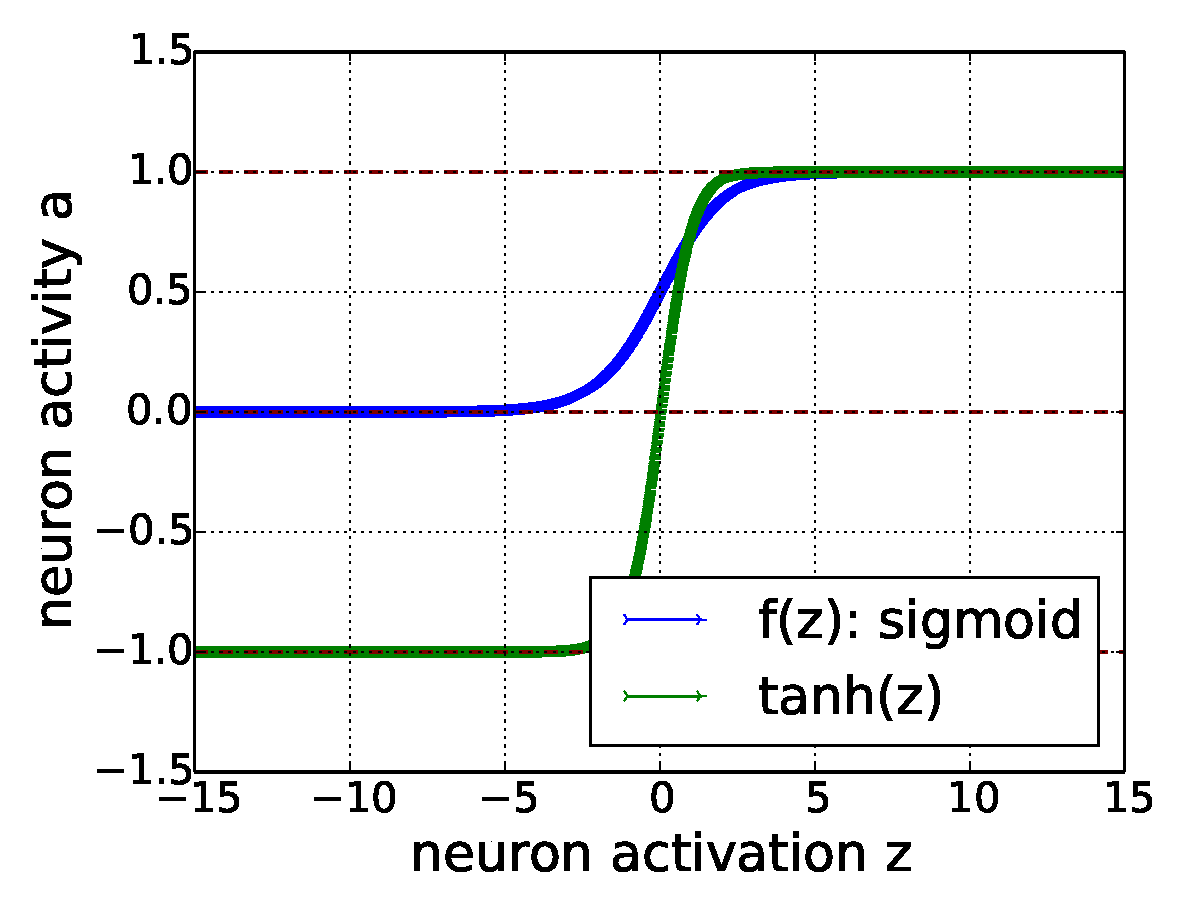
\includegraphics[width=0.7\textwidth]{transfer_functions.eps}
%  \caption{Transfer functions: \textit{Sigmoid} and \textit{Tanh}}
%  \label{fig:methods:transfer_functions}
%\end{figure}

\section{Automatic Speech recognition}

ASR (Automatic speech recognition) is a way of converting sound into text. 

Sound is nothing more than vibrations of the air that we humans are trained exceptionally well to decode. Moreover, now, we are teaching our computers how to do this. In the beginning, we have a stream of words that a person has uttered. The sound is picked up by a microphone and converted to a digital signal through a sound card, which means a stream of ones and zeroes.

The first step the ASR system need to do is process the sound. It steps the sound to have chunks of speech (shown in \cref{fig:chunked_voice}) that can be worked with and that can be mapped to letters. These chunks are called phones. 

\begin{figure}[H]
    \centering
    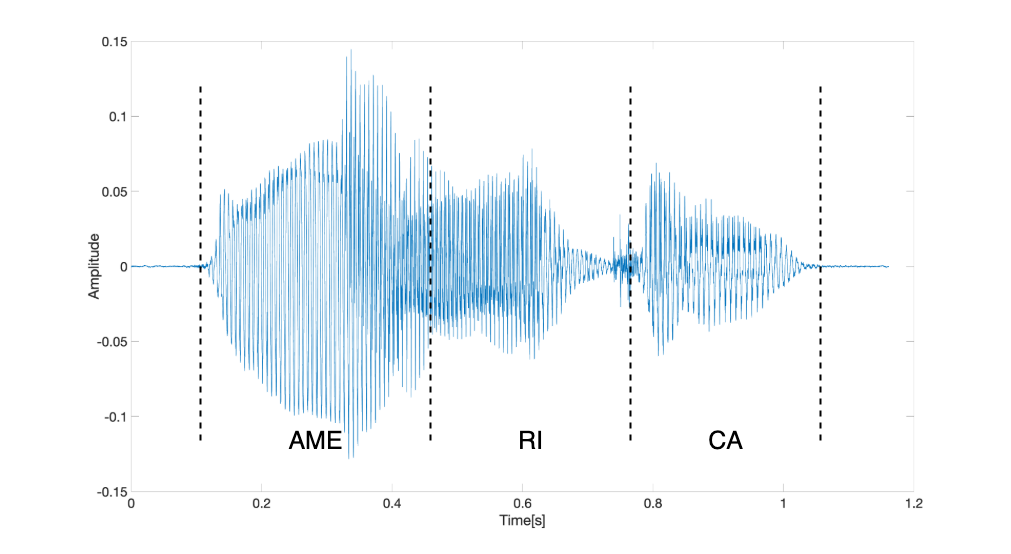
\includegraphics[width=\textwidth]{img/voice_edit.png}
    \caption{Chunked voice}
    \label{fig:chunked_voice}
\end{figure}

The part of ASR responsible for mapping sound to phones is called the acoustic model as a set of building blocks, boxes which contain models for all phones in a given language as showing \cref{fig:phones_boxes}.

\begin{figure}[H]
    \centering
    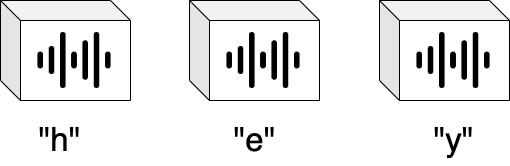
\includegraphics[width=0.7\textwidth]{img/phones_boxes.png}
    \caption{Phones boxes}
    \label{fig:phones_boxes}
\end{figure}

There are boxes labelled, for example, A, B, C, depending on which phones are used in the particular language. On top of that, part of this construction set is also contextual probabilities. It means how likely a phone is to follow another. The acoustic model's task is to guess which phones have pronounced and how they combine into a word. The acoustic model processes the sound and compares it to the models of individual phones from its boxes. Since speech is very complex in a real scenario, the chunks that a person uttered will be similar to more than one box. The acoustic model takes this into account and also looks at the neighbouring chunks and their contextual probabilities. For example, string "HELLO" the first sound that a person uttered might have been H. However, it also could have been CH. The second sound looks most like E, but it could have been \begin{IPA}@\end{IPA} , A or even I, with different degrees of certainty. The next sound is probably L, but it also could be R. There are different probabilities of these phones in context, for example, H followed by E is more likely, at least in English, than H followed by I. The ASR system combines these bits of information and outputs the most likely result - a string of phones.\citep{stanislav_petr_2020}

The next step is to convert it into words. Nevertheless, this part can be tricky because the ASR does not know when a word starts or ends. Contrary to popular belief, there are no pauses between words in fluent speech. This particular string "heloumaj..." of phones can constitute several different phrases, for example, "hell oh my nay miss" or "hello mine aim is", or "hello my name is". The part of ASR responsible for mapping phones to words and phrases is called the language model.

Hidden Markov Models are widely used for the statistical approach for automatic speech recognition. Suppose that W=**** is a sequence of words, and O=**** is a sequence of phones. These sequences are taken with a period of 10 ms for segments of speech of length from 20 to 40 ms. To figure out a task to guess which phones have pronounced and how they combine into a word is used Bayes Theorem for conditional probability.

\begin{equation}
    \boldsymbol{W}^{\prime}=\underset{w}{\operatorname{argmax}} P(\boldsymbol{W} \mid \boldsymbol{O})=\underset{w}{\operatorname{argmax}} \frac{P(\boldsymbol{W}) P(\boldsymbol{O} \mid \boldsymbol{W})}{P(\boldsymbol{O})}
\end{equation}

Where P(W) is the a priori probability of word W, P(O|W) is the probability that the sequence of phones O will be generated under the conditions of pronouncing the sequence of words W, P(O) is the a priori probability of the sequence of phones O. 

Since the probability P(O) is independent of the sequence of words W, it is possible to modify the equation into the form:

\begin{equation}
    \boldsymbol{W}^{\prime}=\underset{w}{\operatorname{argmax}} P(\boldsymbol{W} \mid \boldsymbol{O})=\underset{w}{\operatorname{argmax}} P(\boldsymbol{W}) P(\boldsymbol{O} \mid \boldsymbol{W})
\end{equation}

\section{TextToSpeech - synthesis}

The task of generating speech out of text information has originally two approaches:
\begin{enumerate}
    \item Concatenative (unit selection)
    \item Statistical parametric
\end{enumerate}

With concatenative synthesis is based on sequential combining of shot prerecorded samples of speech. These samples can be stored in a database in the form of whole sentences, phrases, words and different phonemes. It depends on the application of the solutions. Building the unit selections synthesis model consists of three steps:

\begin{enumerate}
    \item Recording of whole selected speech units in no possible context.
    \item Labelling segmentation of units.
    \item Choosing the most appropriate units. 
\end{enumerate}

The concatenated method is the most straightforward approach to speech generation. Disadvantages include the requirement to have ample storage for recorded units and an ability to apply various changes to a voice.

Statistical parametric synthesis consists of two parts, as shown in \cref{fig:synthesis_model}.
The training step's approach is to extract excitation parameters like fundamental frequency and dynamic features, and spectral parameters from the speech database. Then we estimate them using one of the statistical models. The Hidden Markov model or HMM is the most widely used for this task. It should be noted that HMM is conscious dependent it means that in this step, in addition to phonetic context, linguistic and prosodic context is taken into account. In the synthesis part, at first given sentence is converted into points with a dependent label sequence, and then their chance HMM is constructed according to this sequence. Next, spectrum and excitation parameters are generated from the utterance HMM, and finally, speech waveforms are synthesized from these parameters using excitation generation and the speech synthesis filter. The advantages of the statistical parametric approach are:
\begin{enumerate}
    \item Small footprint
    \item No need to store speech waveforms, only statistics language independence
    \item Flexibility in changing voice characteristics speaking styles and emotions. 
\end{enumerate}
The most noticeable drawback is the quality of a synthesized speech.

\begin{figure}[H]
    \centering
    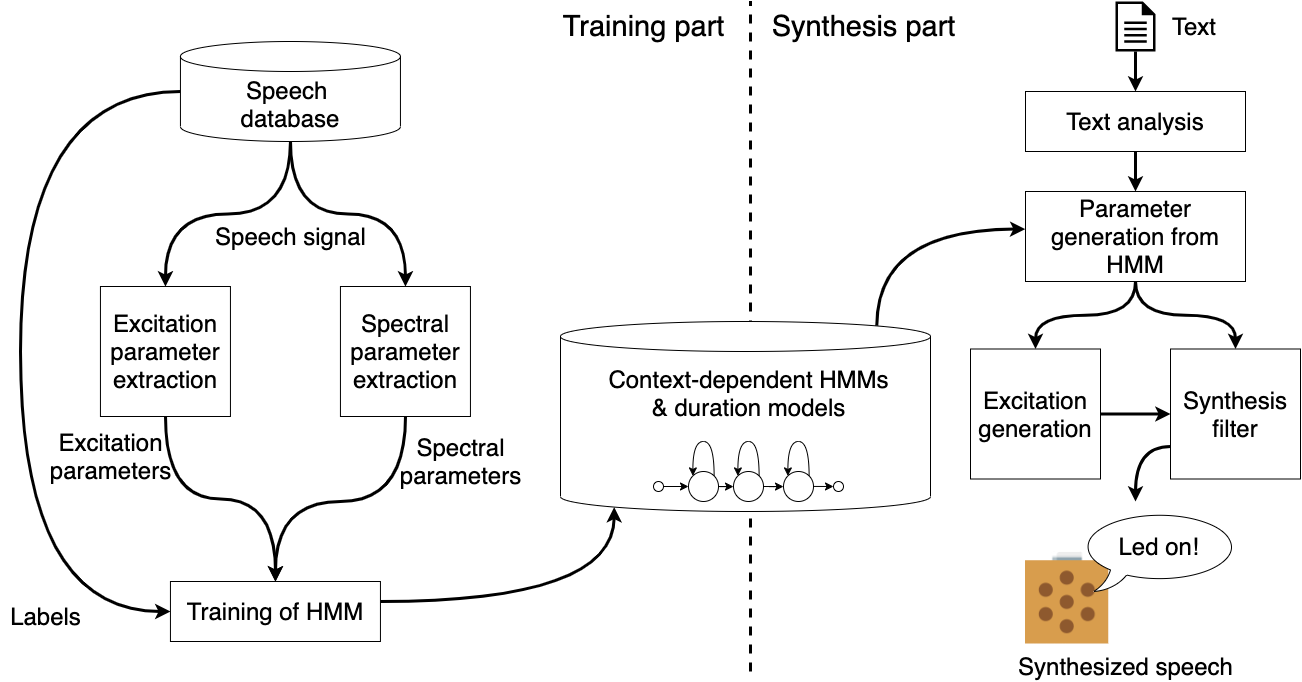
\includegraphics[width=\textwidth]{img/synthesis_model.png}
    \caption{Synthesis model}
    \label{fig:synthesis_model}
\end{figure}


\section{KKY SpeechCloud}

SpeechCloud is a system that connects ASR and TTS systems operating together via one interface. It is then possible to use these systems by many applications simultaneously through this interface. An independent instance is created for each dialogue system, allowing a client to create a characteristic language model, send a speech record to recognize, and receive the synthesized speech.

SpeechCloud provides the same services to all clients, unless otherwise limited or specified. Each client should have the same functions, but each device, experiment or project is separated from the others, so the results are not affected by the unwanted intervention.

The architecture of SpeechCloud and connection to client briefly visualizing \cref{fig:speechcloud_schema}.

SpeechCloud using the module SCAPIServer as a primary point for reach a connection with the client application. Thus, the module negotiates with the client the configuration for client applications, control communication channel, and authentication of a session. SCAPIServer also provides these pieces of information to other modules. The SIPSwitch module mediates the audio data transfer service between the SCWorker component and the client application. One instance of the SCWorker component is reserved for each client. This component instance holds one ASR and TTS instance. The SCWorker component has access to a TCP/IP network connection to obtain additional data sources.

\begin{figure}[H]
    \centering
    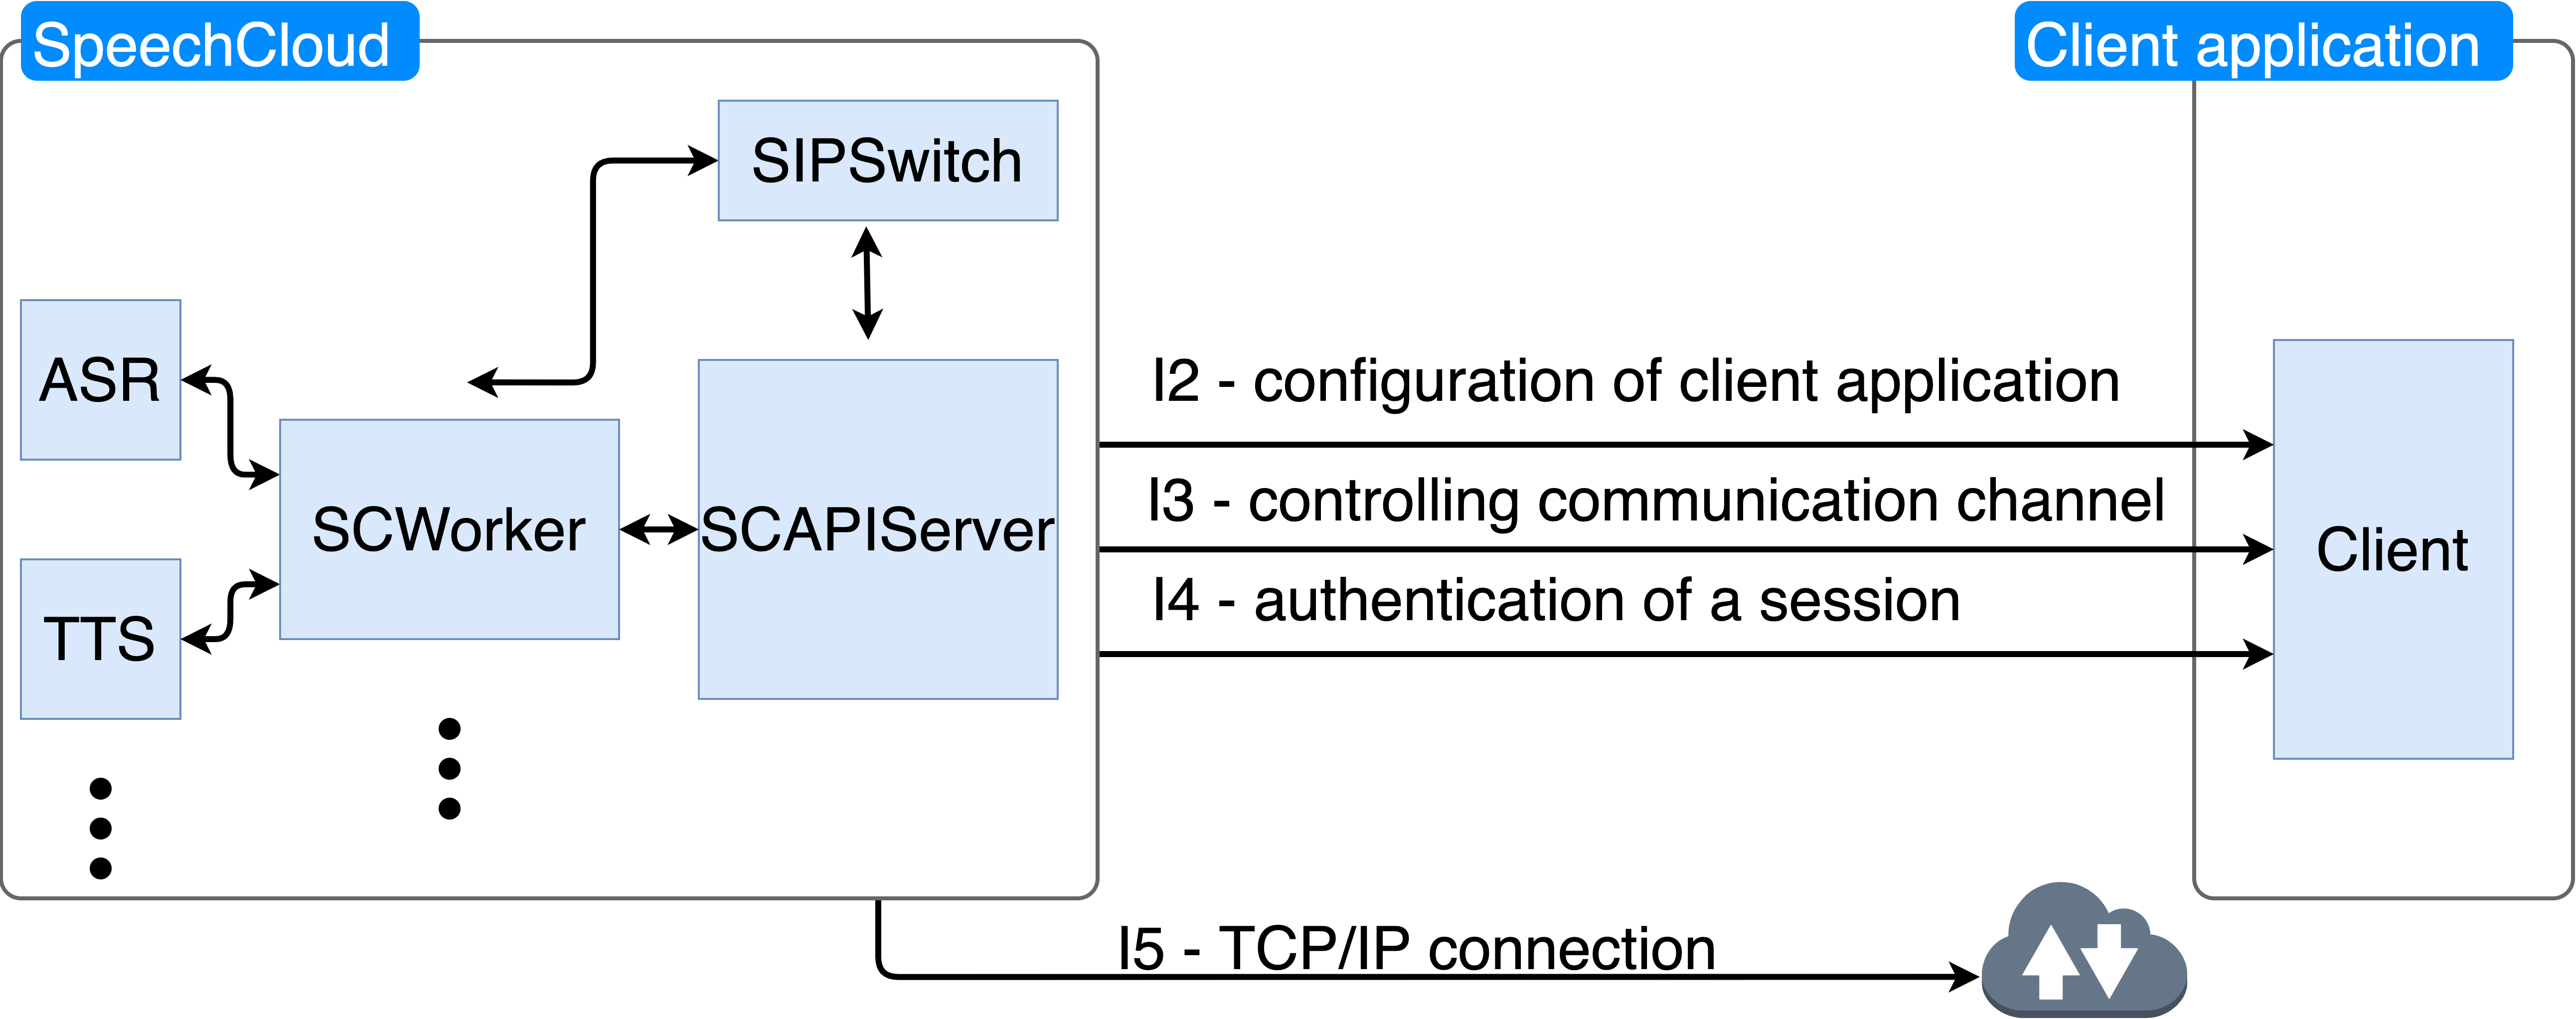
\includegraphics[width=\textwidth]{img/speechcloud_schema.png}
    \caption{SpeechCloud schema}
    \label{fig:speechcloud_schema}
\end{figure}

Solving the subject of the connection and transmission of data via Internet communication protocols is not the content of this work hence are used ready-made software components.